\section {Frontend - Android Client}
The following section will describe the product the front-end team developed during the course.
The product consists of two different applications: Elephant, the web browser, and an implementation
of the NetInf services that support Information-Centric Networking.

\subsection{Elephant Web Browser}
The web browser application is a basic implementation of a web browser that lets the user browse
the web. The graphical interface is very simple and intuitive, since the only steps required for
opening a web page is to tap on the address bar, enter the desired web page and confirm the input URL.
This is achieved by either pressing enter on the keyboard or tapping on the refresh button on the right
of the address bar. At this point the browser will start to communicate with the NetInfService to
search for the resources that are contained in the requested web page.

While loading a web page the browser gives the user continuous feedback in the form of a spinning wheel,
indicating that the resources contained in the web page are being downloaded.
Resources refer to content of a web page, such as pictures or texts.
What is interesting to observe is that the spinning wheel changes color while loading a web page,
indicating what kind of transmission is being used to retrieve each specific resource.
The application uses five different colors: gray to indicate that a search is in progress, red to indicate
that a resource is retrieved by the uplink connection (3G or WIFI), green to indicate database activity,
black to indicate the use of a NRS caching node, and finally blue when a device retrieves a resource from
another device via Bluetooth. The application also offers the possibility to interrupt the
loading process by tapping on the the same icon used to start loading a page, as it toggles between a refresh
icon and cancel icon. \fig{loaded_page} shows an example view of the web browser.\\

\begin{figure}
\centering
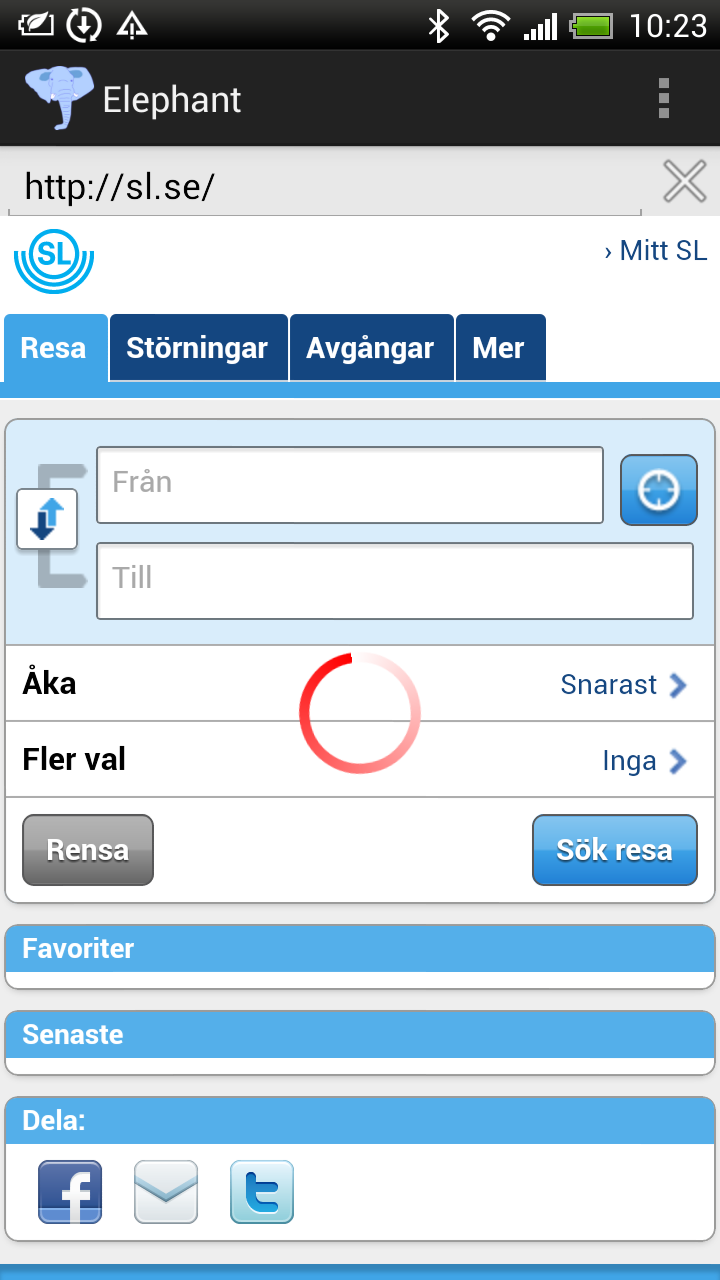
\includegraphics[scale=0.29]{img/loaded_page.png}
\caption{Loading a web page via uplink}\label{fig:loaded_page}
\end{figure}

To make sure that Elephant will be able to retrive resources from an NRS caching node and to be able
to connect to other devices via Bluetooth, the NetInfService application has to be up and running.
This is because the NetInf services enable communication to other nodes in the system and keep
track of which devices have a certain resource to serve via Bluetooth.

Elephant contains some customizable settings that can be found in the menu entry on the top right of the application.
These settings make it possible to take advantage of the NetInf services. In comparison to other
available browsers, Elephant makes use of Information-Centric Networking instead of Location-Based Networking
in an attempt to lower network congestion.
Since one of the core ideas of Information-Centric Networking is to share content between nodes, the setting page
tries to present a simple and transparent way to exploit the underlying capabilities of the NetInf services.
The user can decide if she wants to share visited pages, and also if she wants to upload web pages to a caching node.
The first menu entry gives the possibility to register the local device as a locator that can serve other devices
with the loaded content via Bluetooth.
Enabling the second menu entry the device will not only register you as a locator, but will also transfer the actual bytes,
so that the content can be served by a NRS cache node if there is one available.

The last menu entry for the setting is for opening the NetInf Services' settings, so that the user does not have to switch applications
manually for changing the service settings.
\newpage

\begin{figure}
\centering
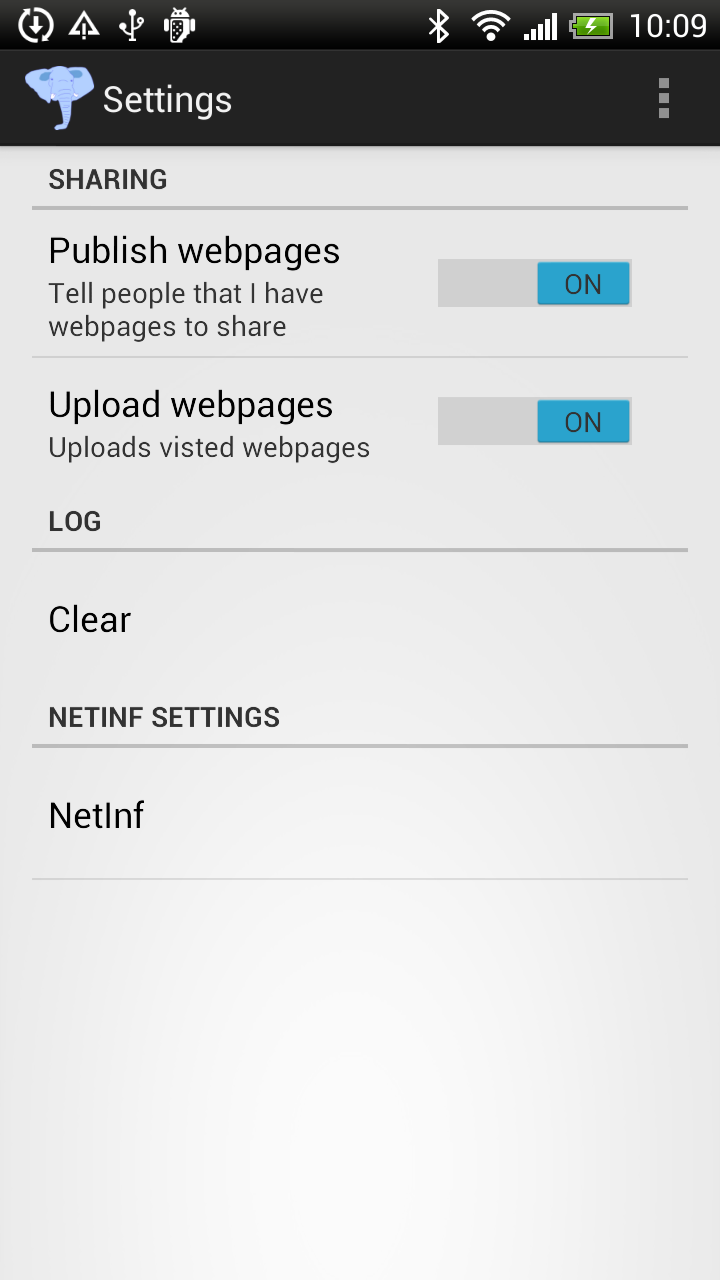
\includegraphics[scale=0.29]{img/ele_settings.png}
\caption{Settings view of Elephant}\label{fig:ele_settings}
\end{figure}

\newpage
Finally, \fig{help} shows a simple help view presenting a brief description of the functionalities of the application,
so that the user can have a better understanding of how the web browser works.\\

\begin{figure}
\centering
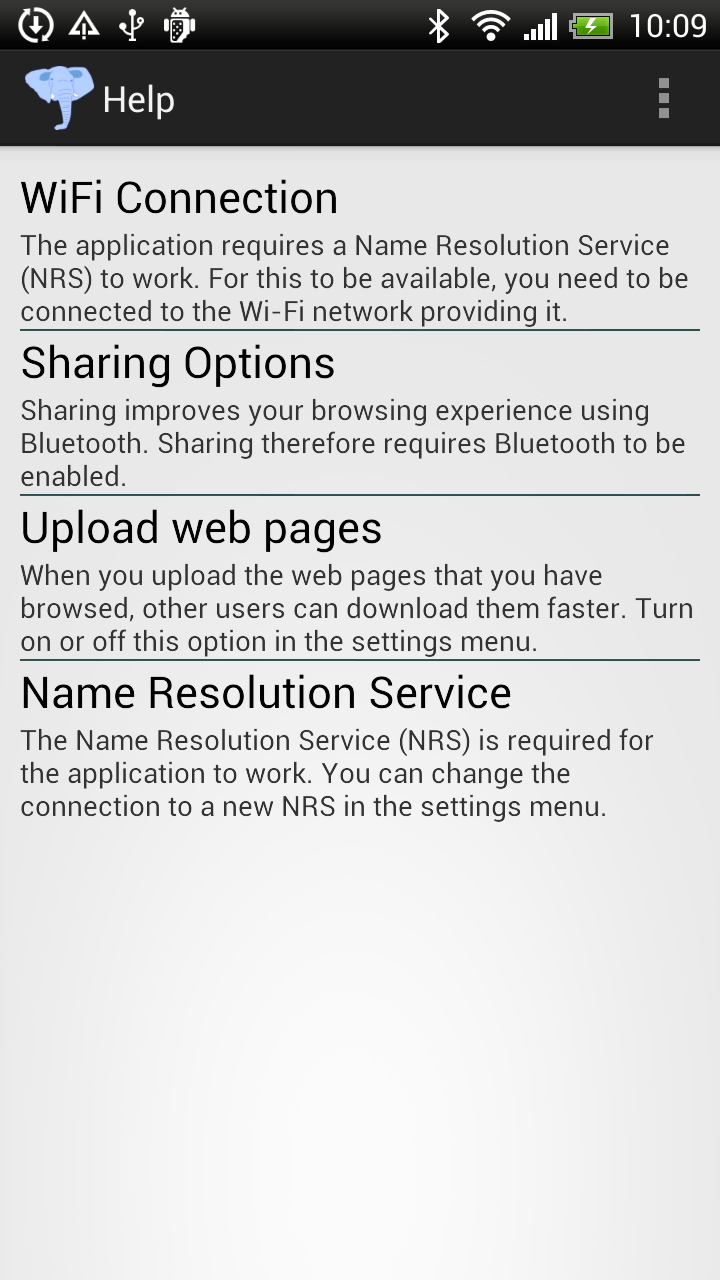
\includegraphics[scale=0.29]{img/help.png}
\caption{Help view}\label{fig:help}
\end{figure}

\subsection{NetInfService}

\begin{table}
\centering
 \begin{tabular}{|c|p{10cm}|}\hline
  Functionality	& Description \\\hline
  Search	& The application searches for the hash value of the resource requested, specified by a URL. This search includes
		  searching for the hash value within the local database and the remote Name Resolution Service (NRS).
		  It returns the value, if found.\\\hline
  Get		& A Get request that contains the hash value of an Information Object (IO) triggers a content retrieval of the
		  corresponding resource. The application tries to retrieve the content either from the Local Resolution Service (LRS), the NRS
		  or from a remote Bluetooth device.\\\hline
  Publish	& The application can register the local device as a locator for a resource specified by a hash in the NRS. This way, remote
		  devices can try to retrieve that resource from the local device using Bluetooth. \\\hline
  Full put	& The full put is a publish request that contains the actual content corresponding to the resource that is published. Thus,
		  the NRS, to which the local device is connected to, can store the content and serve it itself.\\\hline
		  
 \end{tabular}
  \caption{Functionalities}\label{tab:netinffunctionalities}
\end{table}

The NetInfService is a stand-alone application that can be used by other
applications in order to make use of Information-Centric Networking. All functionalities
that are provided are listed in \tab{netinffunctionalities}. If an application
needs our services, the NetInf Service application has to run in background.\\

\begin{figure}
\centering
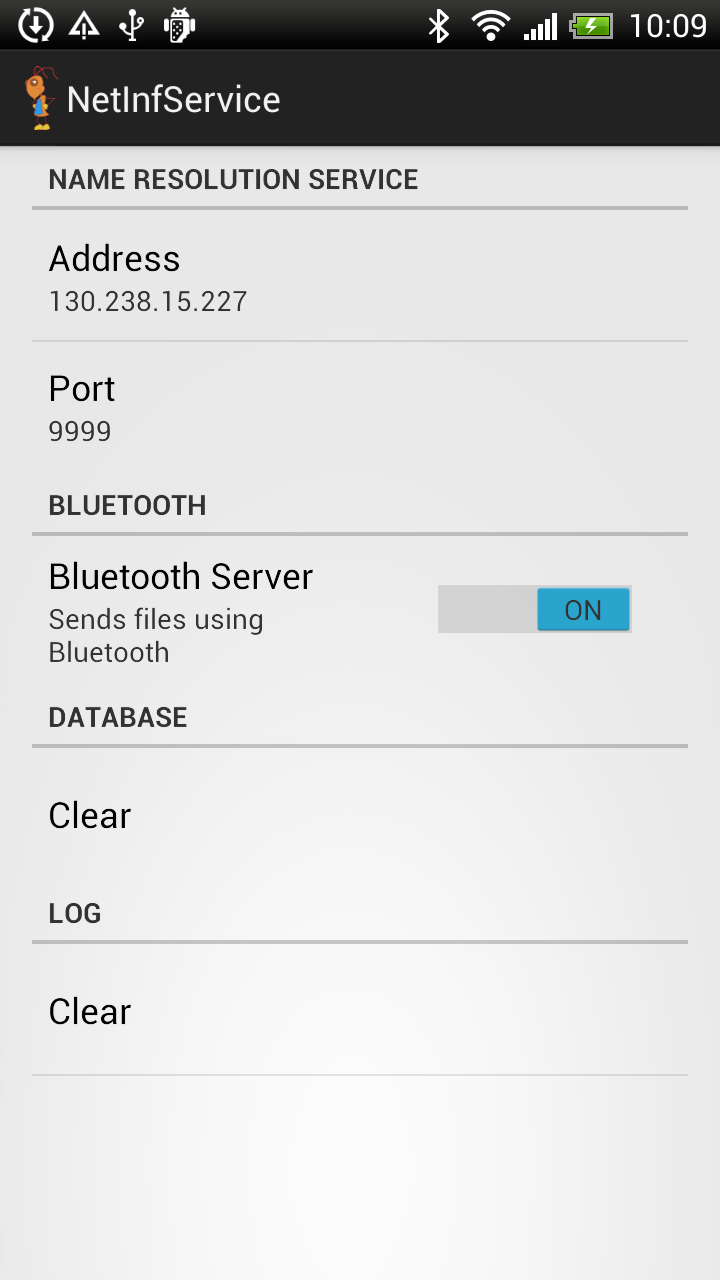
\includegraphics[scale=0.29]{img/ant_settings.png}
\caption{NetInf Service Settings}\label{fig:servicesettings}
\end{figure}

The services are configurable within a simple and self-explanatory user interface that is shown in \fig{servicesettings}.
If a user wants to change the NRS her device is communicating with, the address as well as the port can be changed accordingly.
In addition a user can decide whether she wants to share her downloaded content with other remote devices. Only if the \textit{Bluetooth Server} 
is turned on, data will be shared.
Finally, the database as well as the logs created during the run can be cleared.
The database stores every single resource that is published. At some point, the database will contain a huge amount of old data that is not
usable anymore. Clearing the database will then improve the run time since the search among stored content will perform faster.
Log files are used for debugging purposes. In case a log is old, clear it and rerun the application in order to 
gain new logs.
